% !TeX spellcheck = en_GB

In this chapter we want to show the different cost rasters, that were created from the same set of layers at different resolutions.
The Least Cost Path is estimated from this set of rasters.
In the last step the Least Cost Path is computed from the lower resolution rasters and compared with the Least Cost Paths computed from a high resolution raster.

\subsection{Cost Raster}\label{subsec:cost-raster}

The cost raster contains all the costs for the geographical region of the study area.
%%The surrounding of the study area, uses a no-data value and will not be use for the calculation of the Least Cost Path.
The different cost layers in the study area are aggregated by the maximum function.
If the resolution is higher than the object size, then the effect of the rasterisation with all touched True or False is limited.
For all touched True any part of the pixel that is covered by the object, will attribute that whole pixel to the object.
This makes the object appear a halve a pixel size larger in all directs.
As can be seen in figure~\ref{fig:costs_5m}, which shows a detailed view of the costs for the village of Beverstedt.
 %% Due to the maximum aggregation of the costs, the average cost of the raster of all touched true will be over estimated.
The rasterisation with all touched false will be a better description of the real size of the object, for high resolution.
\begin{figure}
	\centering

	\subfloat[\centering All touched: True.]{{\includegraphics[width=.45\linewidth]{./images/CostRaster_5m_alT_v2_small.png} }}%
	\qquad
	\subfloat[\centering All touched: False.]{{\includegraphics[width=.45\linewidth]{./images/CostRaster_5m_alF_v2_small.png} }}%
	\caption{Figures of the cost raster. Contrasting the for different values in all touched at a resolution of 5~m.}
	\label{fig:costs_5m}
\end{figure}

In contrast, if the resolution is smaller, than the object-size this behaviour changes.
In general, while the area, of the pixel increases for all touched True, the area for which the cost is overestimated also increases.
As the pixel size for all touched  False increases, not only does the overestimated area increases, but in addition the object is less probable situated in the centre of the pixel. 
Therefore, object is sampled at random.
Hence, all touched false leads to a loss of information for smaller objects.
\todo{Put this part into Discussion?} Since the default cost is much smaller than the average cost, this method underestimates the cost.
The figure~\ref{fig:costs_100m} shows, that for the resolution of 100 m, that larger objects are still included in the map, but appear to be larger.
But smaller objects, such as roads, are not fully or randomly included.
\begin{figure}
	\centering

	\subfloat[\centering All touched: True.]{{\includegraphics[width=.45\linewidth]{./images/CostRaster_100m_alT_v2_small.png} }}%
	\qquad
	\subfloat[\centering All touched: False.]{{\includegraphics[width=.45\linewidth]{./images/CostRaster_100m_alF_v2_small.png} }}%
	\caption{Figures of the cost raster. Contrasting the for different values in all touched at a resolution of 100~m.}
	\label{fig:costs_100m}
\end{figure}
\todo{Put this part into Discussion?}Thus, with having larger areas and more objects, with higher costs, all touched True rasterisation might more likely lead to longer roots and more likely to block the  direct spatial path.

\subsection{Least Cost Paths}\label{subsec:least-cost-paths}
For each resolution the Least Cost Paths were estimated from the all\_touched False and all\_touched True rasters.

For the study, a start point were chosen at a transformer about 6~km north of the container terminal Bremerhaven and an end point at a transformer in the southeast of the Osterholz county. 

The distance of Least Cost Paths of the all touched false to the paths of the all touched true raster is calculated by the mean minimum distance.
For each vertex $P_i$ in the path $L_1$ the minimum distance between the vertex and the path $L_2$
is calculated and then the minimum distances are averaged (see equation~\ref{eq:1}).
\begin{equation}
	\label{eq:1}
	d_{mean} = \frac{1}{|L_1|} \sum_{i=1}^{n} d_{min}(p_i, L_2) \Bigr\vert p_i \in L_1
\end{equation}
This equation is used, to measure the degree of similarity between the paths.

Table~\ref{tab:2} shows the distance between the two paths decreases
with increasing resolution.
In addition, this tendency is depicted in figure~\ref{fig:paths_resolution} for the calculated cost paths of 5~m and 100~m resolutions.


At the same time, the differences in the aggregated costs per resolution remain almost constant.
On one hand it can be seen, that the all\_touched False underestimates the costs and that this tendency scales
linearly with the resolution.
On the other hand, the all\_touched True least cost overestimates the aggregated costs on a linear scale of
the resolution.


\begin{figure}
	\centering

	\subfloat[\centering resolution of 5 m.]{{\includegraphics[width=.45\linewidth]{./images/LeastCostPaths_5m_v2_small.png} }}%
	\qquad
	\subfloat[\centering resolution of 100 m.]{{\includegraphics[width=.45\linewidth]{./images/LeastCostPaths_100m_v2_small.png} }}%
	\caption{Figures of the least cost paths. Contrasting the paths for different resolutions. Paths computed from all touched false raster are indicated by dashed lines. Results from all touched True are indicuated by continuous lines. Higher resolutions are indicated by the color green, lower resolutions by the color red. Using OpenStreetMaps as base map.}
	\label{fig:paths_resolution}
\end{figure}

\begin{figure}
	\centering

	\subfloat[\centering all touched false.]{{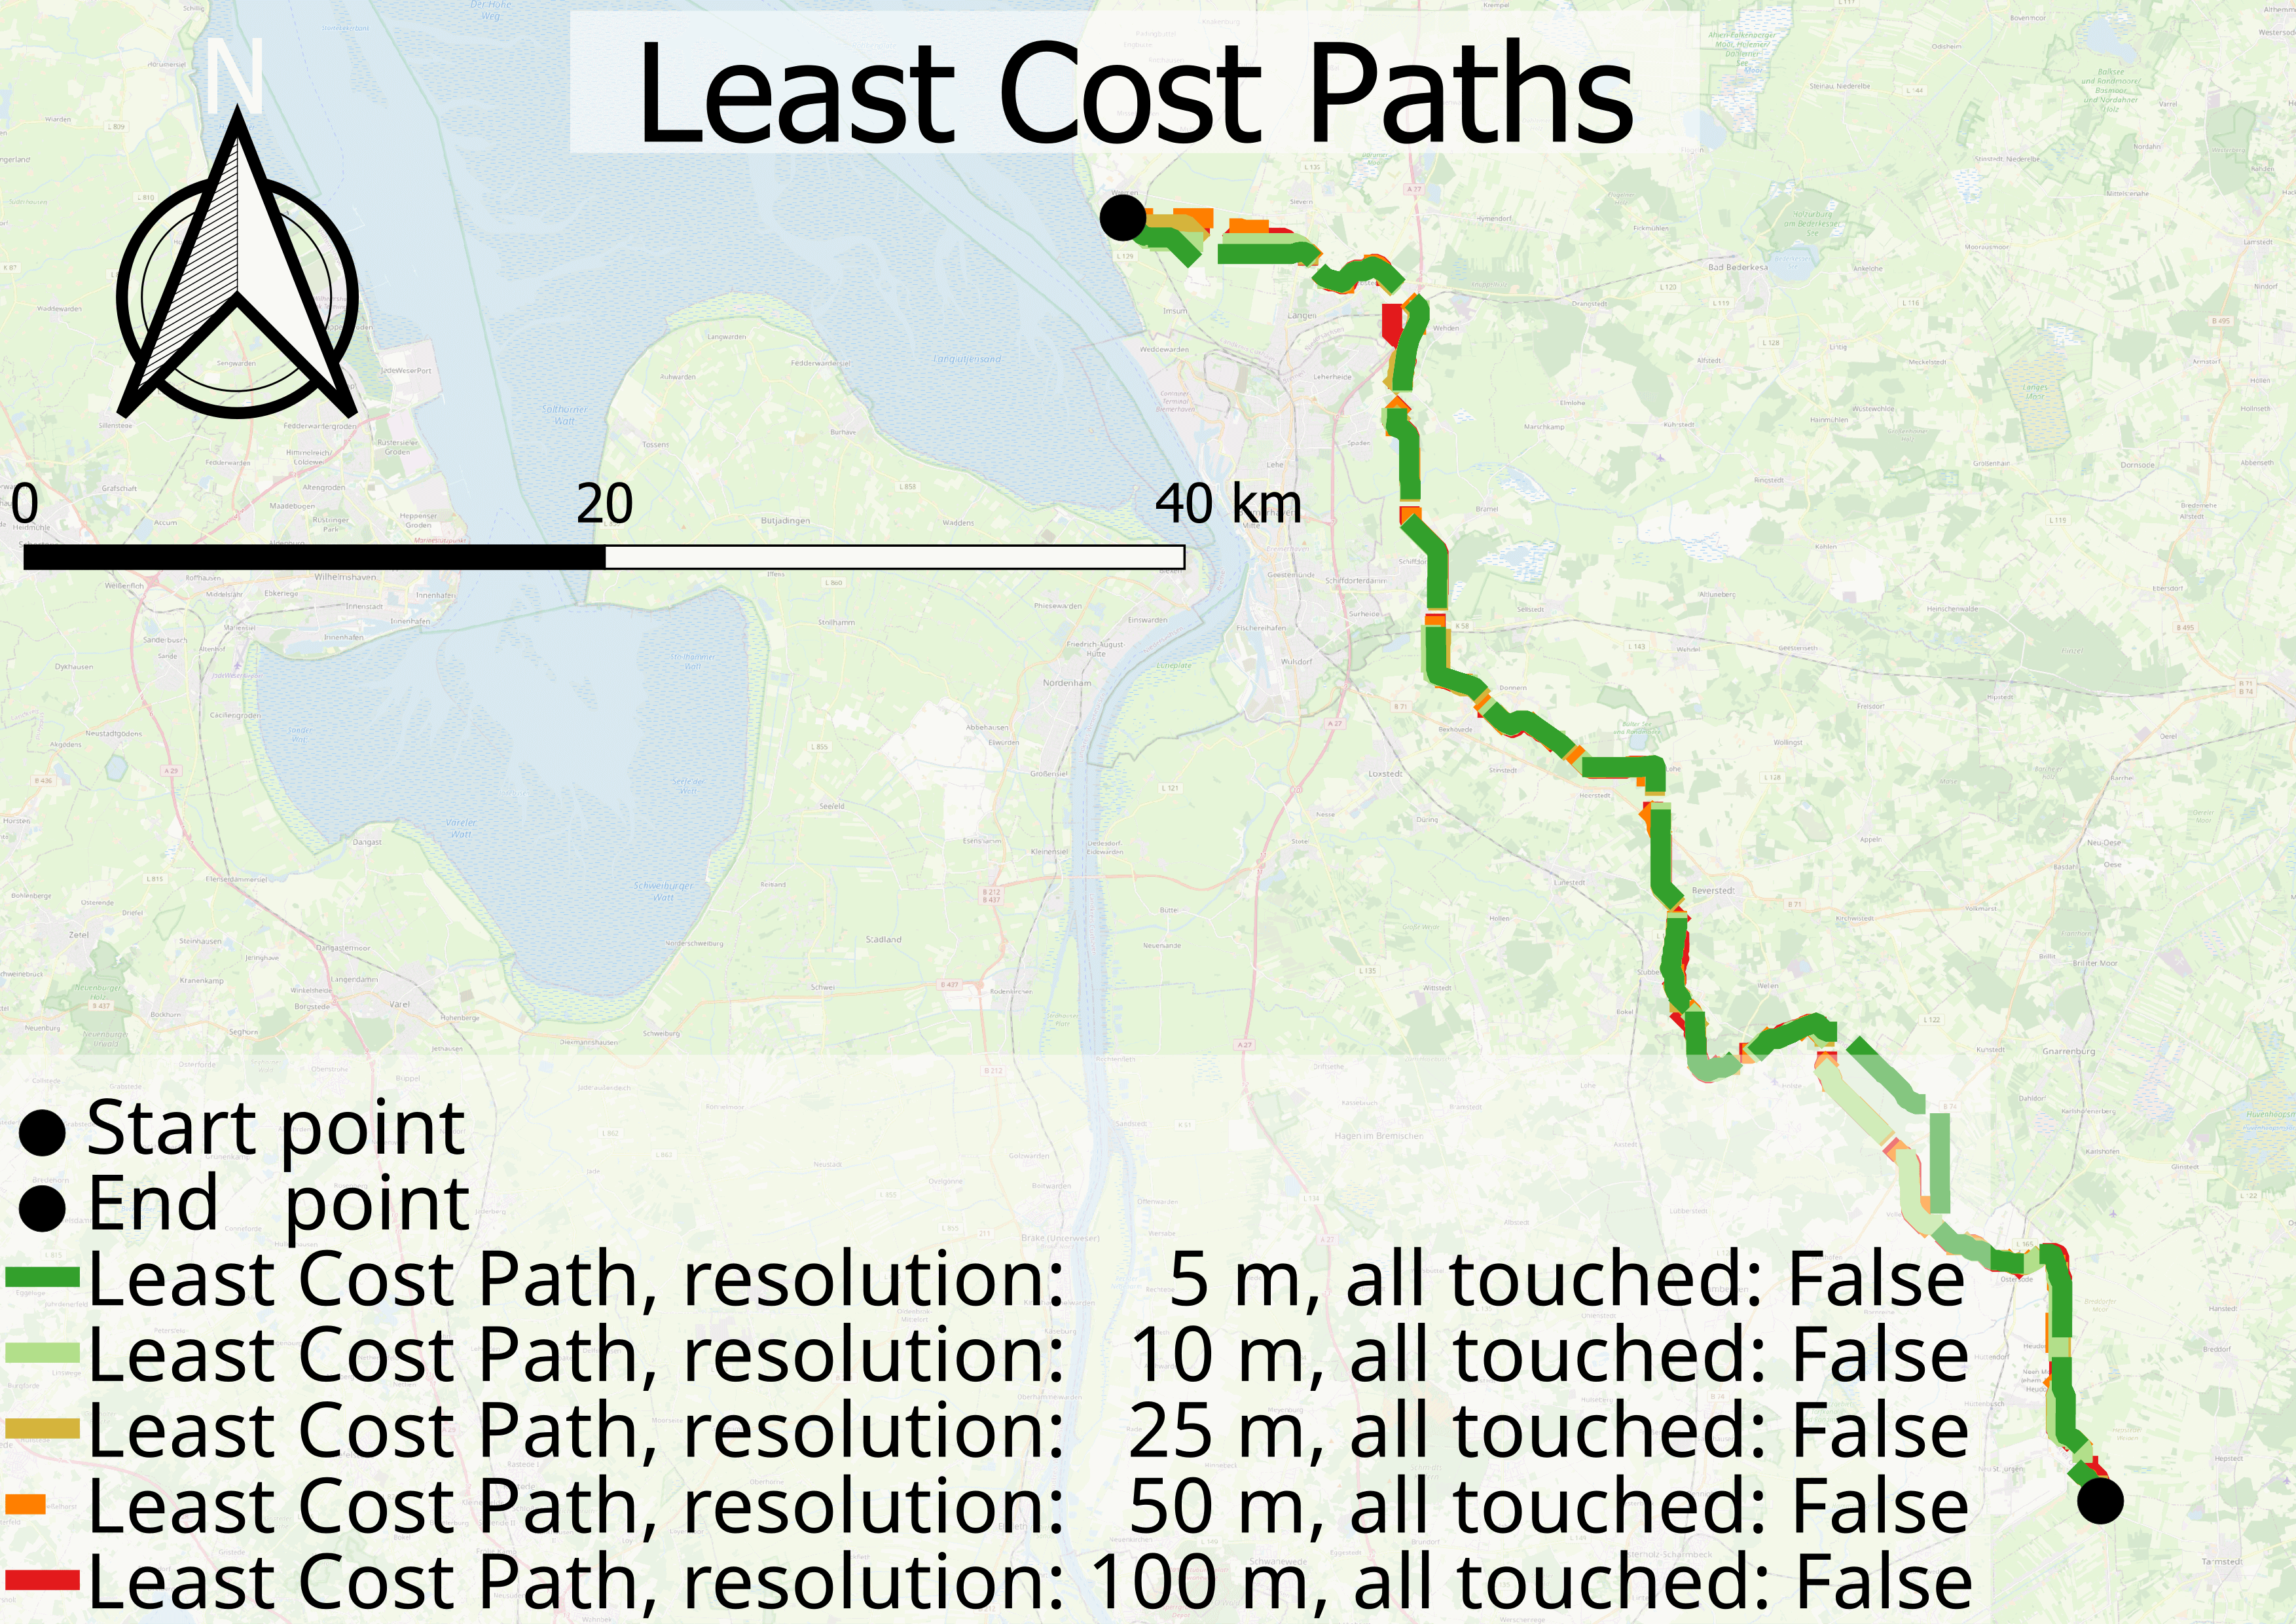
\includegraphics[width=.45\linewidth]{./images/LeastCostPaths_al_F_v2_small.png} }}%
	\qquad
	\subfloat[\centering all touched true.]{{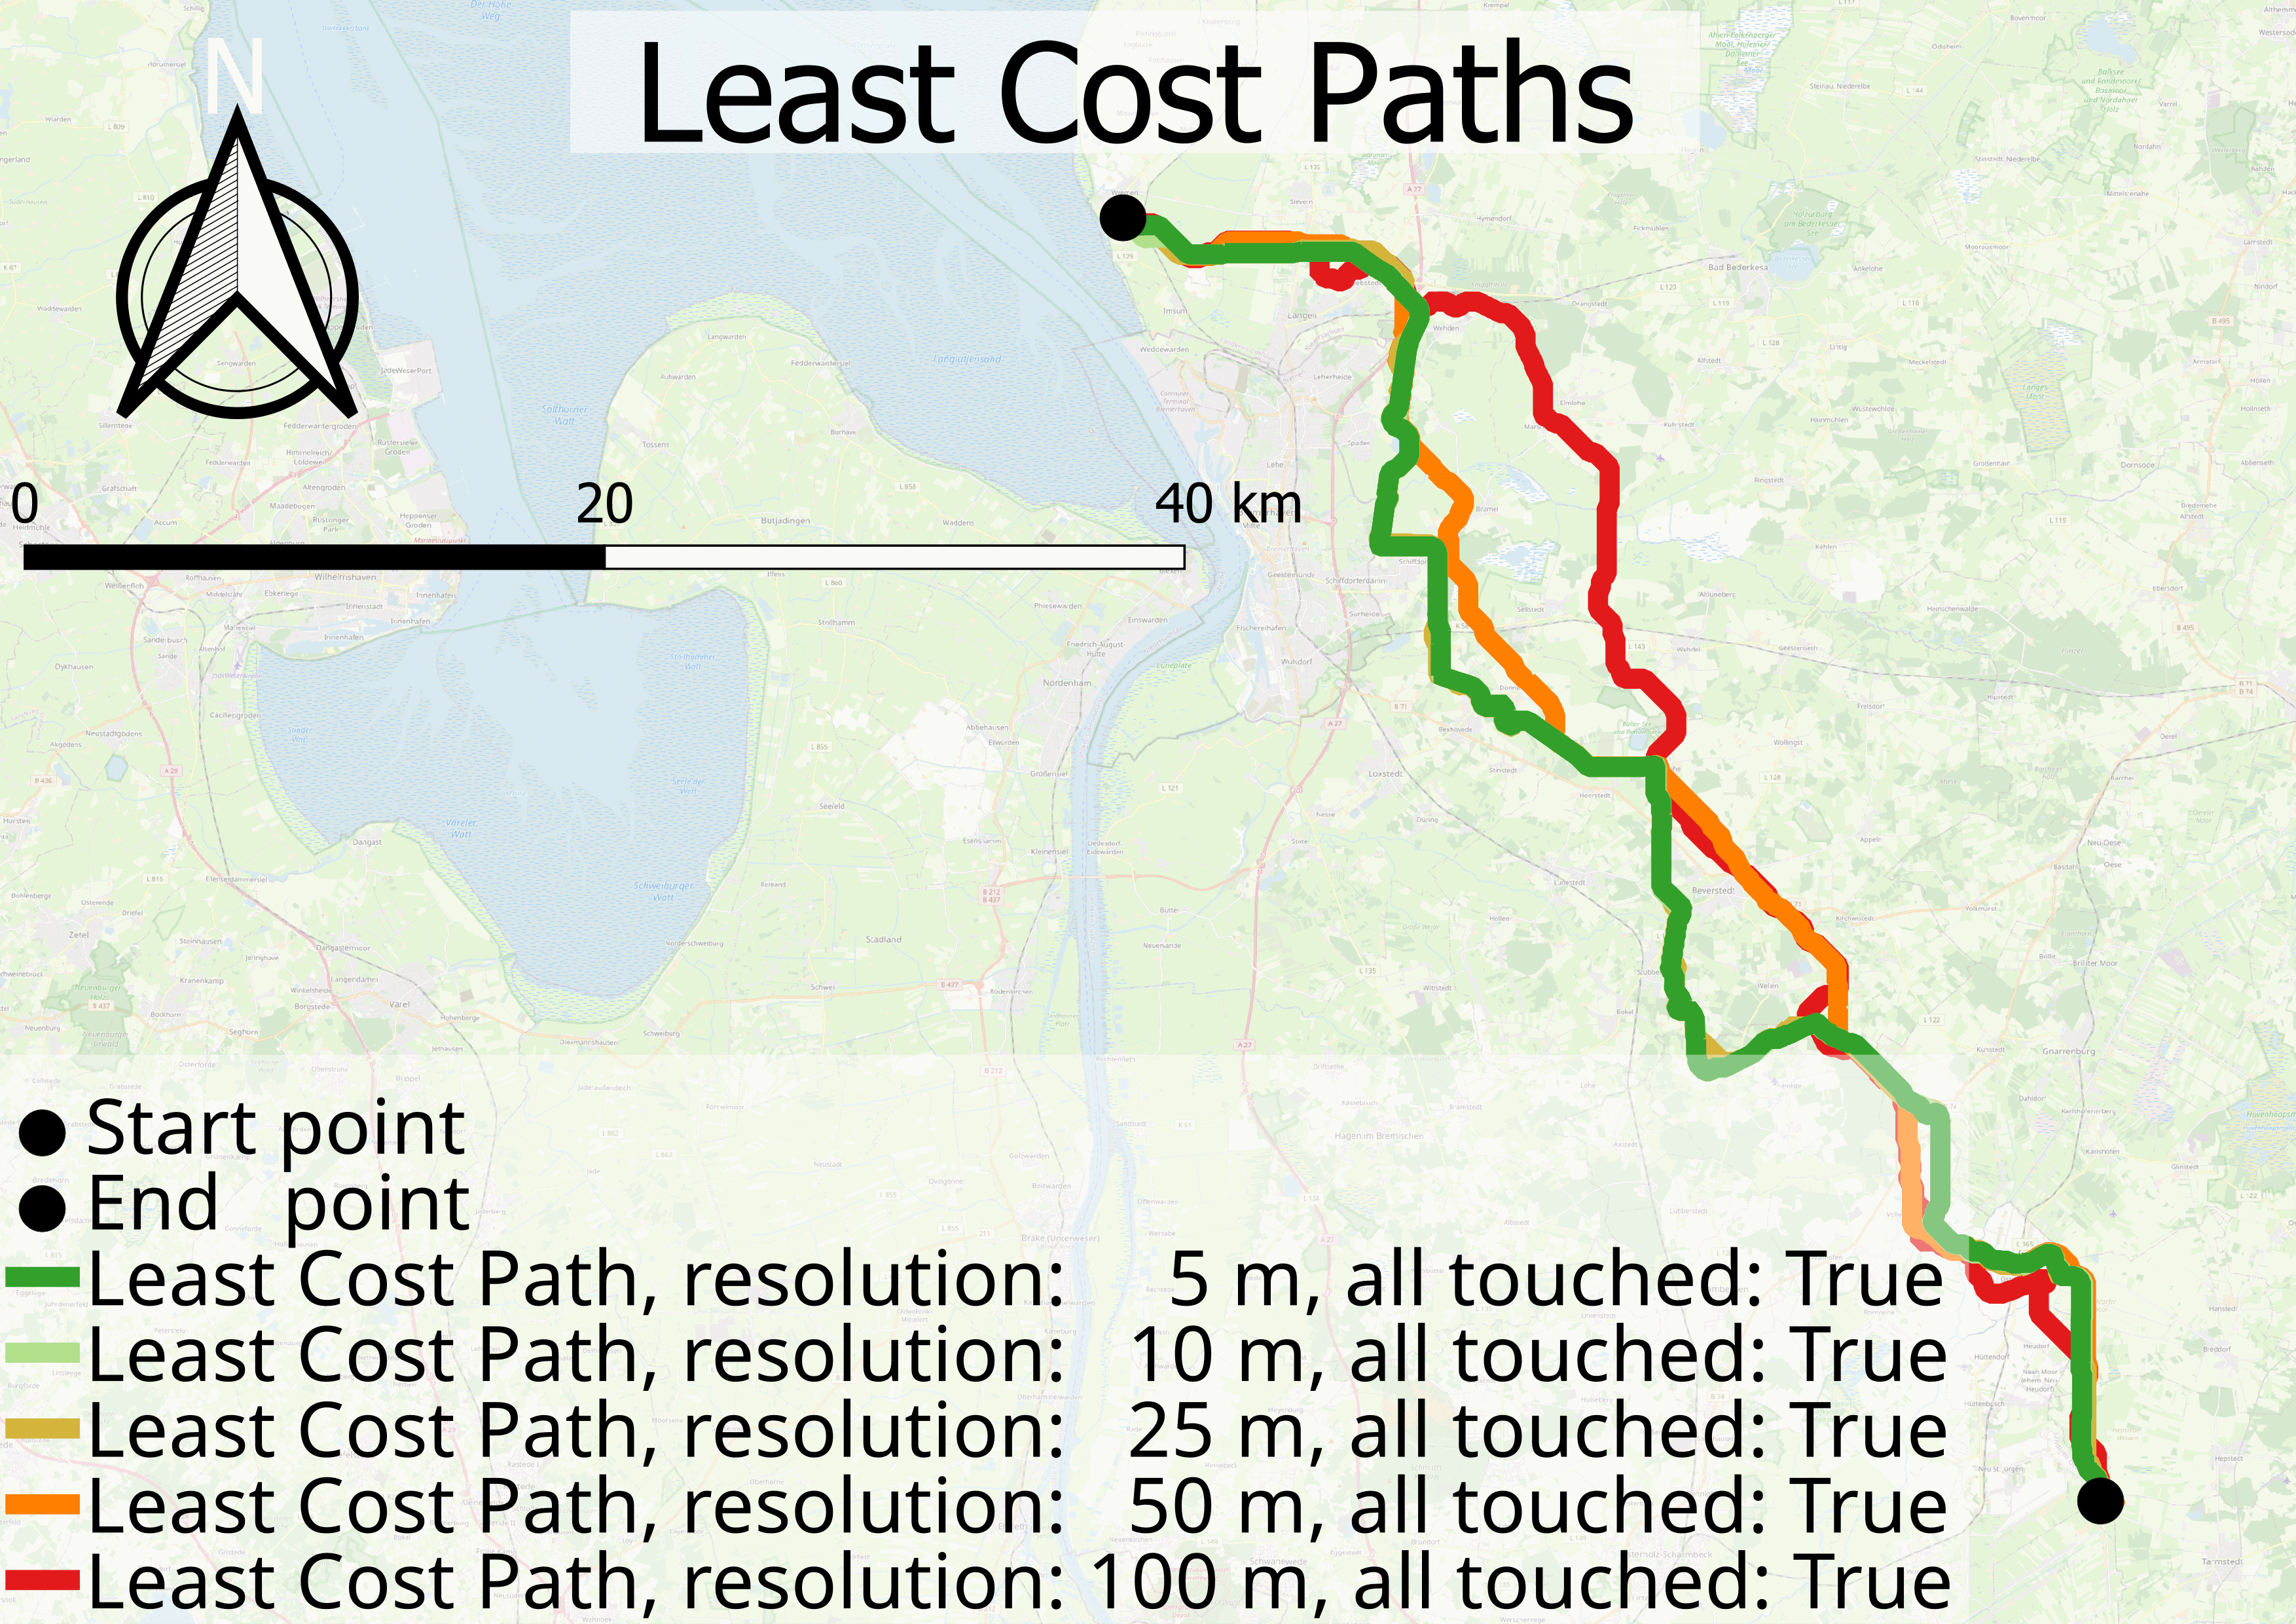
\includegraphics[width=.45\linewidth]{./images/LeastCostPaths_al_T_v2_small.png} }}%

	\caption{Figures of the least cost paths. Contrasting the changes of the least cost paths for the different results, depending on the parameter all\_touched. Paths computed from all touched false raster are indicated by dashed lines. Results from all touched True are indicuated by continuous lines. Higher resolutions are indicated by the color green, lower resolutions by the color red. Using OpenStreetMaps as base map.}
	\label{fig:paths_alltouched}
\end{figure}

\begin{table*}[t]
	\caption{Least cost paths as length for the different resolution of the raster, including the mean minimum distance and the maximum minimum distance and the agg. costs. From the agg. costs the differences of the agg. costs and the agg. costs per resolution are given.} 
	\label{tab:2}
	\centering
	\begin{tabular}{ r  r  r  r  r  r  r  r  r  r}
		res /m & $l_{al=f} /m$ & $l_{al=t} /m$ & $d_{mean}$ /m & $d_{max}/m$ & agg.  $ cost_{al=f}$ & agg. $ cost_{al=t}$ &  $\Delta $ costs & agg. $costs_{al=f} /m$ & agg. $costs_{al=t} /m$ \\
		\hline
		5 	& 76136.3	& 78002.0 &  126.0 & 1065.0 & 18665.9 & 19616.8 & -850.00 & 93329.6 &  97584.8 \\
		10 	& 75430.1 	& 77936.6 &  277.9 & 1590.0 &  8931.2 &  9731.2 & -799.95 & 89312.5 &  97311.8 \\
		25 	& 75422.9 	& 78422.9 &  313.8 & 1621.2 &  3354.9 &  3872.7 & -517.78 & 83871.7 &  96816.4 \\
		50 	& 76135.0	& 70620.0 & 1140.0 & 4950.0 &  1409.0 &  2300.1 & -891.05 & 70451.2 & 115003.7 \\
		100 & 76283.8	& 74120.7 & 1946.4 & 6016.6 &   640.5 &  1572.3 & -931.70 & 64051.6 & 167226.8 \\

	\end{tabular}
\end{table*}

When estimating distance between the Least Costs Paths from all\_touched True rasterisation and all\_touched False at the same resolution 
the mean minimum distance between the 100~m resolution paths is 1946.41~m and between the 5~m resolution paths is 126.04~m.
The similarity for the all touched False paths is higher, than for the all touched true raster.
The distance for the 100~m path to the 5~m resolution path is 243.42~m for all touched false and 2109.44~m for all touched true.

When comparing the similarity between the all touched false paths themselves and the similarity between the all touched false rasters to the all touched true rasters of the same resolution: The similarity in between the all all\_touched False paths is higher than, than for most paths of same resolution.
Namely except for the highest resolution.

This behaviour is shown in figure~\ref{fig:paths_alltouched}.
On a more detailed level, it can be seen, that the paths of all\_touched False also converge directly to the all touched True paths, but the extent is smaller.
The length of the paths only differs by a maximum of about 10 \%.
On the other hand, side the length of the paths can increase, because with more vertices are used with higher resolution.

The zonal stat (see table~\ref{tab:3}) for a buffer of 100~m (5~m) around the path has been used, to estimate the
percentage of each costs levels around the path.
When using all\_touched True rasterisation at higher resolution, the tendency is to use a higher percentage of the
\textit{Preferential Level} and less of the\textit{NoRestriction} Level.
The ratio of the 100~m buffered Least Cost Path, strongly shifted  to Levels lower costs.

There is no strong tendency for the all\_touched False least cost paths.

\subsection{Execution time}\label{subsec:execution-time}

In theory, the execution time increases with the square of the resolution, because higher resolutions result in a higher number of pixels and thus data points the aggregated costs needs to be calculated for. 
A full logarithmic fit for several repetitions of the execution shows, that the execution time scales with power of $2.1997  \pm 0.007$ of the inverse resolution. 

The total execution time consists of two parts. 
The aggregation of the costs and the back tracking of the least cost to find the path.

\setlength{\tabcolsep}{10pt}

\begin{table*}[t]
	\caption{resolution (r) of Category percentages of each least cost path for a buff of 100 m (5 m) around the least cost path.}
	\label{tab:3}
	\centering
	\begin{tabular}{ r  r  r r  r r  r r  r r  r r}
		res /m & all touched & \multicolumn{2}{c}{ $ r_{Preferential} \% $}  & \multicolumn{2}{c}{ $ r_{No Restriction} \% $ }  & \multicolumn{2}{c}{ $ r_{Restricted} \% $}  & \multicolumn{2}{ c }{ $ r_{strongly Restricted}\% $ } & \multicolumn{2}{c}{ $ r_{Prohibited} \% $ } \\
		\hline
		5 & False &  4.7  &  (5.4) & 58.7 & (58.9) & 8.8 & (8.4) & 0.7 & (0.7) & 27.1 & (26.7)  \\
		10 & False &  19.6 & (33.5) & 68.5 & (64.5)  & 1.0 & (0.8) & 0.8 & (0.3) & 10.1 & (0.9)\\
		25 & False &  19.2 & (34.2) & 68.9 & (64.9)  & 1.0 & (0.2) & 0.7 & (0.1) & 9.7 & (0.6)\\
		50 & False &  20.4 & (33.2) & 68.0 & (66.2)  & 0.9 & (0.1) & 0.7 & (0.0) & 10.1 & (0.5)\\
		100 & False &  21.1 & (30.7) & 69.1 & (68.8)  & 1.1 & (0.0) & 0.7 & (0.0) & 7.9 & (0.4) \\

		\hline

		5 & True  &  18.9 & (28.5) & 67.3 & (66.4) & 1.3 & (1.6) & 1.0 & (0.5) & 11.5 & (3.0) \\	
		10 & True &  18.9 & (33.7) & 66.6 & (63.4)  & 1.6 & (1.4) & 1.4 & (0.6) & 11.5 & (1.0)\\	
		25 & True &  18.7 & (31.9) & 65.5 & (65.5)  & 2.0 & (1.3) & 2.5 & (0.7) & 11.4 & (0.6)\\
		50 & True &  9.1 & (13.0) & 75.7 & (83.0) & 3.9 & (2.0) & 4.2 & (1.6) & 7.1 & (0.4) \\
		100 & True &  7.0 & (10.1) & 73.8 & (81.9)  & 5.5 & (3.9) & 8.5 & (3.6) & 5.2 & (0.4) \\	
	\end{tabular}
\end{table*}



\subsection{Faster Processing of the Cost Path Algorithm}\label{subsec:faster-processing-of-the-cost-path-algorithm}

The first step is to optimise the computational speed, by a reduced area.
Another method, is to improve the prediction of the medium resolution itself and thus reduce the need for a computation in higher resolution.

\subsubsection{Compare least cost paths, for overlay of both rasterisations}

For the example paths shown, all touched true rasterisation overestimates the true costs and all touched true underestimates them.

A weighted average of the costs could therefore be a more accurate measure and make estimated medium resolution Least Cost Path more similar, to high resolution paths.
As all example show, the weighting should favour the all touched false raster.
\todo{move to discussion/conclussion:}The best weight should be the percentage of the pixels, which is covered by the object, but this can not be calculated in this work.
An alternative would be to compute the cost raster at a high resolution and reproject them to a medium resolution by a (linear) interpolation of the weights.

\todo{move to planning:}This will speed-up the aggregation.
The time needed for the back tracking stays unchanged.

The optimal ratio of overlaying all touched false and all touched true cost raster for 10~m resolution is estimated via similarity of the resulting Least Cost Path to the path of the original high Resolution raster. 
The mean distance of Least Cost Paths for different ratio is estimated to the path from the all touched false raster of the higher (5~m) resolution. 
Table~\ref{tab:4} shows, that the distance decreases, with increasing ratio (1:1, 2:1, 4:1) and after this optimum is reached, increases with increasing ratio (8:1, 16:1 and so on).
Comparing  the similarity of the paths from the rasters of the different ratios to normal paths with 10~m resolution, paths with a higher ratio of all touched true is nearer to the all touched true paths.
Paths with a ratio in favour of all touched false are much closer to the all touched false paths.


\begin{table}[h!]
	\caption{Length of the path computed from the overlaying of all touched false and true raster and the mean distance of the paths to the paths calculated from the all touched false 5~m resolution  and all touched false and true raster of 10~m resolution.}
	\label{tab:4}
	\centering
	\begin{tabular}{ r  r  r  r}
		r & $d_{5~al=f}$ /m &  $d_{10~al=f}$ /m & $d_{10~al=t}$ /m \\
		\hline
		
		  1:1  &    119.6 &  285.5 &  47.2\\
		  2:1  &    97.1 &  263.5 &  74.2\\
		  4:1  &    40.1 &  206.4 & 100.2\\
		  8:1  &    41.7 &  169.0 & 137.3\\
		 16:1  &    56.7 &  153.3 & 152.72\\
		 32:1  &    56.7 &  145.6 & 162.1\\
		 64:1  &   163.5 &   10.6 & 272.4\\
	  % 128:1  &   163.80 &   10.3 & 276.7\\
		
	\end{tabular}
\end{table}


\subsubsection{Compare least cost paths, for down sampled cost paths}

As an alternative to the superposition of the all touched true and false rasters for the same resolution, the all touched false raster is down-sampling to 10~m, 25~m, 50~m and 100~m (with bi-linear) interpolation.
With this method, smaller structures can still be fully seen in the cost raster, although the resolution is reduced.
The distances of the paths that are computed from the bi-linear down sampled raster to the path of the original 5~m resolution (all touched false) shows (see table~\ref{tab:5}), that only down-sampling to a resolution of 10~m, produces a path that is relatively close the high resolution path.

The opposite is true for the lower resolution raster which is more similar to paths computed from the all touched true cost raster.
Every path from a down sampled raster is more similar to a path computed from an all touched true raster, than an all touched false raster, although the all touched false raster of the 5 m resolution was used for down sampling.\todo{interpretation all touched true and downsampling, both show all details, but downsampling, more similar to original geometry}

\begin{table}[h!]
	\caption{Length of the path computed from the bi-linear down sampled raster and the mean distance of the paths from the down sampled raster to the paths calculated from the all touched true and all touched false raster of the same resolution as the down sampled raster.}
	\label{tab:5}
	\centering
	\begin{tabular}{ r  r  r  r  r}
		res /m & l /m  & $d_{5~m}$ /m &  $d_{al=f}$ /m & $d_{al=t}$ /m \\
		\hline
		
		10  & 75980.6 &    59.3 &  219.4 & 143.6\\
		25  & 70205.3 &   385.8 &  558.1 & 432.8\\
		50  & 69217.9 &   730.8 &  693.4 & 255.7\\
		100 & 66667.9 &  1681.3 & 1605.6 & 400.6\\
		
	\end{tabular}
\end{table}


% \subsubsection{Restrict search to a minimum sized bounding box}
\subsubsection{Restrict search to a buffered around the least cost paths}



Construct a polygon from the two Least Cost Paths (all touched true and all touched false of the same resolution).
Buffer the polygon with twice the maximum  minimum path distance  (see equation~\ref{eq:2}).
\begin{equation}
	\label{eq:2}
	d_{max} = max(\sum_{i=1}^{n} d_{min}(p_i, L_2)) \Bigr\vert p_i \in L_1
\end{equation}


This provided the possibility  to run a 2.5~m resolution cost raster and clip it to the extent of the polygon. 
This clipped 2.5~m raster for all touched true changed the path only slightly change. 

The all touched False raster, on the other hand, leads to a completely new previously unused subroute at the end of the path.
Due to the low resolution a small path became passable.
This small path is a power line next to road between protected landscape areas.
The road and the protected landscape area are both \textit{restricted} areas, while the power line is \textit{preferred}.
This shows, that the way the cost raster is created in the first place can play a crucial role, in the end result.
So that a nuance, can cause a detour.
When this behaviour occurs, the polygon may not include the Least Cost Path.
\todo{move: discussion}This polygon should therefore be overlapped with a polygon around the shortest path.


%\subsubsection{Restrict search to reachable points}
%For this purpose the aggregated cost as to converted back into a raster.

\subsubsection{Examine the proposed solutions}
To broaden the view and verify the result, e.g.\ start and end points, four different routes should be found using the above strategies.
Two routes should be found form the start point to two new points in the south east of the investigated area and two routes should be found from the north and north east of the study area to the end point.

For three of the four routes, the Least Cost Path estimation from the clipped raster, was able to calculated exactly the same result.
For the fourth path, the Least Cost Path from the 5~m resolution raster was clipped out by the buffer around the 50~m resolution paths.
The speed up from the clipping of the higher resolution raster depends on the number of pixels that, have been clipped. 

Bi-linear down sampling the of the high resolution raster to a medium resolution, did not result in any benefits compared to an original medium resolution raster.
The aggregated cost per resolution of the Least Cost Path from the down-sampled raster is higher, than that from the higher resolution 5~m raster and the normal medium resolution 10~m raster.
In addition, the distance from these paths to the high resolution path  is greater, than the distance from the original 10~m resolution path to the 5~m resolution path (see table~\ref{tab:6}).
\todo{interpretation: Why is the down-sampling result so different? Don't know.}

\begin{table}[h!]
	\caption{Length of the path, the resolution corrected costs and the mean distance to the path created from the 5~m resolution all touched false raster for the four control routes, for the reference path of constructed from the 5~m  and 10~m raster and the down 5~m to 10~m down sampled raster and the 5~m clipped raster.}
	\label{tab:6}
	\centering
	\begin{tabular}{ r @{\hspace*{3mm}}  r  r  r  r}
		Route & Method & $length /m$ & $costs_{al=f}$ & $d_{mean}$ /m \\
		\hline
		P1-E & 5~m 			& 107889.6 & 208547.8 &        \\
		 	 & Clipped 		& 107889.6 & 208547.8 &   0.0  \\
		 	 & Down			&  96754.2 & 212911.0 & 628.1 \\
		 	 & 10~m 		& 107232.9 & 203010.2 & 103.5 \\
		\hline
		P2-E & 5~m 			& 103706.4 & 155567.9 &        \\
		 	 & Clipped 		& 103706.4 & 155567.9 &   0.0 \\
		 	 & Down 	    &  92403.3 & 158238.6	& 639.9 \\
		 	 & 10~m 		& 104249.9 & 149899.7 & 177.7 \\
		\hline
		S-P3 & 5~m 			& 102187.1 & 34503.8 	&         \\
			 & Clipped 		&  90377.1 & 37926.1 	& 4465.4 \\
			 & Down 	    &  94125.6 & 37574.9 	&  742.4 \\
			 & 10~m 		& 102461.6 & 32446.0 	&   81.2 \\
		\hline
		S-P4 & 5~m 			& 96449.2 	& 33865.5 	&  		\\
		 	 & Clipped 		& 96449.2 	& 33865.5 	& 0.0 	\\
			 & Down 		& 87861.1 	& 36462.7 	& 796.4\\
			 & 10~m 		& 96739.5 	& 31899.3	& 83.5 \\

		
	\end{tabular}
\end{table}



